\documentclass{beamer}
\usepackage[utf8]{inputenc}

\usetheme{Madrid}
\usecolortheme{default}
\usepackage{amsmath,amssymb,amsfonts,amsthm}
\usepackage{txfonts}
\usepackage{tkz-euclide}
\usepackage{listings}
\usepackage{adjustbox}
\usepackage{array}
\usepackage{tabularx}
\usepackage{gvv}
\usepackage{lmodern}
\usepackage{circuitikz}
\usepackage{tikz}
\usepackage{graphicx}
\usepackage{caption}
\captionsetup{labelformat=empty}  % removes "Figure:"


\setbeamertemplate{page number in head/foot}[totalframenumber]

\usepackage{tcolorbox}
\tcbuselibrary{minted,breakable,xparse,skins}



\definecolor{bg}{gray}{0.95}
\DeclareTCBListing{mintedbox}{O{}m!O{}}{%
	breakable=true,
	listing engine=minted,
	listing only,
	minted language=#2,
	minted style=default,
	minted options={%
		linenos,
		gobble=0,
		breaklines=true,
		breakafter=,,
		fontsize=\small,
		numbersep=8pt,
		#1},
	boxsep=0pt,
	left skip=0pt,
	right skip=0pt,
	left=25pt,
	right=0pt,
	top=3pt,
	bottom=3pt,
	arc=5pt,
	leftrule=0pt,
	rightrule=0pt,
	bottomrule=2pt,
	toprule=2pt,
	colback=bg,
	colframe=orange!70,
	enhanced,
	overlay={%
		\begin{tcbclipinterior}
			\fill[orange!20!white] (frame.south west) rectangle ([xshift=20pt]frame.north west);
	\end{tcbclipinterior}},
	#3,
}
\lstset{
	language=C,
	basicstyle=\ttfamily\small,
	keywordstyle=\color{blue},
	stringstyle=\color{orange},
	commentstyle=\color{green!60!black},
	numbers=left,
	numberstyle=\tiny\color{gray},
	breaklines=true,
	showstringspaces=false,
}
\begin{document}

\title 
{1.8.23}
\date{september 13,2025}

\author 
{ADUDOTLA SRIVIDYA - EE25BTECH11006}
\graphicspath{./figs}


\frame{\titlepage}
\begin{frame}{Question}
If the point $\textbf{A}(2,-4)$ is equidistant from $\textbf{P}(3,8)$ and $\textbf{Q}(-10,y)$, find the values of $y$.
 Also find distance $\vec{PQ}$.

 \begin{table}[h!]
    \centering
    \begin{tabular}{|c|c|}
        \hline
        Point & Coordinates \\
        \hline
	    $A$ & $\myvec{1\\-1}$ \\
	    $B$ & $\myvec{-4\\2k}$ \\
	    $C$ & $\myvec{-k\\-5}$ \\
        \hline
    \end{tabular}
    \caption{Vertices of $\triangle ABC$ before substituting $k$}
    \label{tab:triangle_k}
\end{table}

\end{frame}

\begin{frame}{Theoretical Solution}
Since $\vec{A}$ is equidistant from $\vec{P}$ and $\vec{Q}$,

\begin{align}
    \norm{\myvec{\vec{A} - \vec{P}}} = \norm{\myvec{\vec{A} - \vec{Q}}}
\end{align}

\begin{align}
     \norm{\myvec{\vec{A} - \vec{P}}}^2 = \norm{\myvec{\vec{A} - \vec{Q}}}^2
\end{align}

\begin{align}
    {(\vec{A} - \vec{P})}^\top (\vec{A} - \vec{P}) \, &= \, {(\vec{A} - \vec{Q})}^\top (\vec{A} - \vec{Q})
\end{align}

\begin{align}
 {||\vec{A}||}^2 \, - \, 2\vec{A}^\top\vec{P} \, + \, {||\vec{P}||}^2 \, = \, {||\vec{A}||}^2 \, - \, 2\vec{A}^\top\vec{Q} \, + \, {||\vec{Q}||}^2
\end{align}

\end{frame}

\begin{frame}
\begin{align}
    {(\vec{P} - \vec{Q})}^\top \vec{A} \, &= \, \frac{{||\vec{P}||}^2\, - \, {||\vec{Q}||}^2}{2}
\end{align}

\begin{align}
    \myvec{3-(-10)\\8-y}^\top\myvec{2\\-4}\, = \, \frac{73-(-10)^2 -y^2}{2}
\end{align}

\begin{align}
    y^2 +8y + 15 = 0
\end{align}

Therefore,
\begin{align}
    y \, = -5 , -3
\end{align}

\begin{align}
   \vec{Q_1} = \myvec{-10 \\ -5}, \quad
   \vec{Q_2} = \myvec{-10 \\ -3}
\end{align}
\end{frame}

\begin{frame}{Distance}
\begin{align}
    \norm{\myvec{\vec{P} - \vec{Q_1}}} &= \left\|\myvec{3\\8} - \myvec{-10\\-5}\right\| \\
    &= \left\|\myvec{13\\13}\right\| \\
    &= 13\sqrt{2}
\end{align}

\begin{align}
    \norm{\myvec{\vec{P} - \vec{Q_2}}} &= \left\|\myvec{3\\8} - \myvec{-10\\-3}\right\| \\
    &= \left\|\myvec{13\\11}\right\| \\
    &= \sqrt{290}
\end{align}

\end{frame}

\begin{frame}[fragile]{C code}
\begin{lstlisting}
 #include <stdio.h>
#include <math.h>
int main() {
    int Ax = 2, Ay = -4;
    int Px = 3, Py = 8;
    int Qx = -10;
     // Quadratic from ||A-P||^2 = ||A-Q||^2
     // (Ax - Px)^2 + (Ay - Py)^2 = (Ax - Qx)^2 + (Ay - y)^2
    int a = 1, b = 8, c = 15;
    int discrim = b*b - 4*a*c;
    int y1 = (-b + (int)sqrt(discrim)) / (2*a);
    int y2 = (-b - (int)sqrt(discrim)) / (2*a);
    // Distance ||P-Q|| for each y
    double d1 = sqrt((Px - Qx)*(Px - Qx) + (Py - y1)*(Py - y1));
    double d2 = sqrt((Px - Qx)*(Px - Qx) + (Py - y2)*(Py - y2));
    return 0;
}
\end{lstlisting}    
\end{frame}

\begin{frame}[fragile]{Call C.py}
\begin{lstlisting}
import subprocess

# Compile the C program (only once)
subprocess.run(["gcc", "equidistant.c", "-o", "equidistant", "-lm"])

# Run the compiled program and capture output
result = subprocess.run(["./equidistant"], capture_output=True, text=True)

print("Output from C program:")
print(result.stdout)
\end{lstlisting}
\end{frame}

\begin{frame}[fragile]{Plot.py}
\begin{lstlisting}
import matplotlib.pyplot as plt
# Points
A = (2, -4)
P = (3, 8)
Q1 = (-10, -5)
Q2 = (-10, -3)
# Plot points with markers
plt.scatter(*A, color='red', s=100, marker='o', label='A(2,-4)')
plt.scatter(*P, color='blue', s=100, marker='o', label='P(3,8)')
plt.scatter(*Q1, color='green', s=100, marker='o', label='Q(-10,-5)')
plt.scatter(*Q2, color='purple', s=100, marker='o', label='Q2(-10,-3)')
# Draw lines AP, AQ1, AQ2
plt.plot([A[0], P[0]], [A[1], P[1]], 'b--')
plt.plot([A[0], Q1[0]], [A[1], Q1[1]], 'g--')
plt.plot([A[0], Q2[0]], [A[1], Q2[1]], 'm--')
\end{lstlisting}
\end{frame}

\begin{frame}[fragile]{Plot.py}
\begin{lstlisting}
# Annotate points
plt.text(A[0]+0.2, A[1], "A(2,-4)", fontsize=10, color='red')
plt.text(P[0]+0.2, P[1], "P(3,8)", fontsize=10, color='blue')
plt.text(Q1[0]+0.2, Q1[1], "Q1(-10,-5)", fontsize=10, color='green')
plt.text(Q2[0]-1, Q2[1], "Q2(-10,-3)", fontsize=10, color='purple')

# Labels and grid
plt.xlabel('X-axis') 
plt.ylabel('Y-axis')
plt.title('Equidistant Points from A') 
plt.legend()
plt.grid(True)
plt.axhline(0, color='black', linewidth=0.5) 
plt.axvline(0, color='black', linewidth=0.5)

plt.show()
\end{lstlisting}
\end{frame}

\begin{frame}{Plot}
   \begin{figure}[H]
\centering
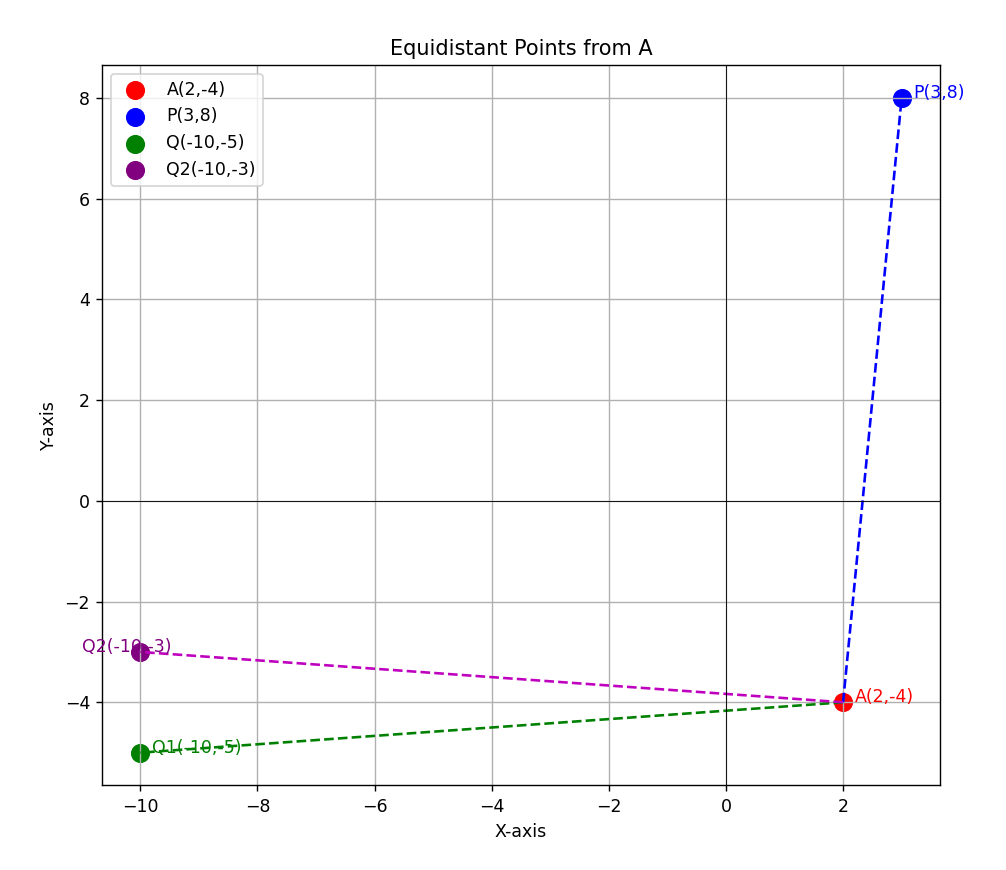
\includegraphics[width=0.6\columnwidth]{../beamer/figs/fig1.png}
 \caption*{Equidistant Points from $\vec{A}$}
\label{fig:graph.png}
\end{figure}
\end{frame}

\end{document}